\thispagestyle{headandfoot}
\begin{center} {\large Verifica��o I}
\end{center}
\vspace{0.5cm} Nome:\rule{14cm}{0.01cm} \\



\vspace{1 cm}
 
{\bf S\'o ser\~ao aceitas respostas devidamente justificadas.}

\vspace{1 cm}
\begin{questions}
\question[3.0] Considere uma part�cula em um po�o infinito localizado
entre 0 e $a$, descrito
pela fun��o de onda em $t=0$: $\psi(x,0)=-A x (x-a/2)$ se $0<x<a/2$ e 
zero nos demais casos.. 
\begin{parts}
  \item Determine o valor da constante de normaliza��o $A$
 \item Calcule a incerteza na posi��o.
  \item Qual � a probabilide em uma medida de energia encontrar o
    sistema no segundo  estado excitado. 
\end{parts}

\question[2.0] Considere a fun��o:

$$\psi(x,t)=A e ^{-a m x^2/\hbar -ikx}$$

\begin{parts}
  \item Determine $A$.
  \item Escreva a fun��o de onda no espa�o de momento
  \item Estime a incerteza no momento.
\end{parts}




\question[2.0] Considere o potencial abaixo e part�culas incidindo com
$V_1<E<V_2$ no sentido do eixo $x$.

\begin{center}
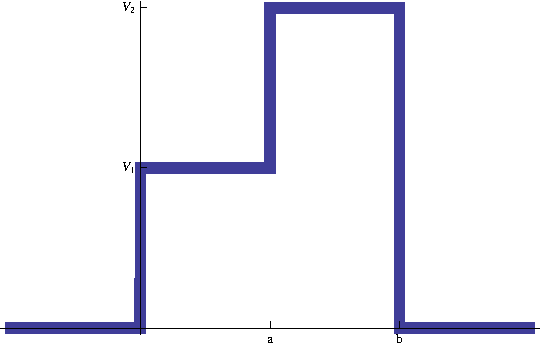
\includegraphics{/Users/neylemke/tex/ensino/mq/potencialex.pdf}
\end{center}
\begin{parts}
  \item Escreva as equa��es de que a fun��o de onda e sua derivada
    devem obedecer.
  \item Use a a aproxima��o WKB para estimar o coeficiente de
    transmiss�o $|T|^2$. 
\end{parts}


\question[2.0] Mostre que 
$$\frac{d}{dt}\int_{-\infty}^\infty \psi_1^* \psi_2dx=0$$
para quaisquer fun��es de onda $\psi_1$ e $\psi_2$ solu��es da equa��o
de Schr�dinger.


\question[Extra]  No dia 5 de maio o Internacional se sagrou
  tricampe�o ga�cho. 
  \begin{parts}
    \item Quem foi o her�i da final antecipada do campeonato?
    \item Quem comando o Internacional em mais essa vit�ria em sua
      extensa galeria de t�tulos?
  \end{parts}
\end{questions}




%%% Local Variables: 
%%% mode: latex
%%% TeX-master: "exame"
%%% TeX-master: "exame"
%%% TeX-master: "exame"
%%% TeX-master: "exame"
%%% End: 
